\section{Latency of blocks that get stuck early}

The overall CMS production resources consist of a highly
interconnected pool of WLCG sites of different capacities and
belonging to different Tier levels. All of them are actively used in
processing/production activities, and an efficient and closely
monitored data transfer system on this complex topology is
essential. It is not unexpected that, in exploiting this heterogeneous
set of resources over long periods of time, some permanent or
transient errors due to hardware/software problems are
experienced. Although CMS tries hard to detect the problematic sites
in advance and proactively takes measures to use them only if they are
safe both for processing and for data transfers, it is not always
possible to select with 100\% purity on long periods of time a subset
consisting of only sites in perfect shape. Hence, it is expected that
the overall transfer system needs to always deal with a bunch of
problematic sites that should nevertheless be used as either source or
destination of some data transfer tasks. In many of these cases, as
the problem may just be at the infrastructural site level, these kind
of transfers show up as “stuck” in the very beginning, i.e. even in
the transfer of the very first file.

\begin{figure}[htp]
\centering
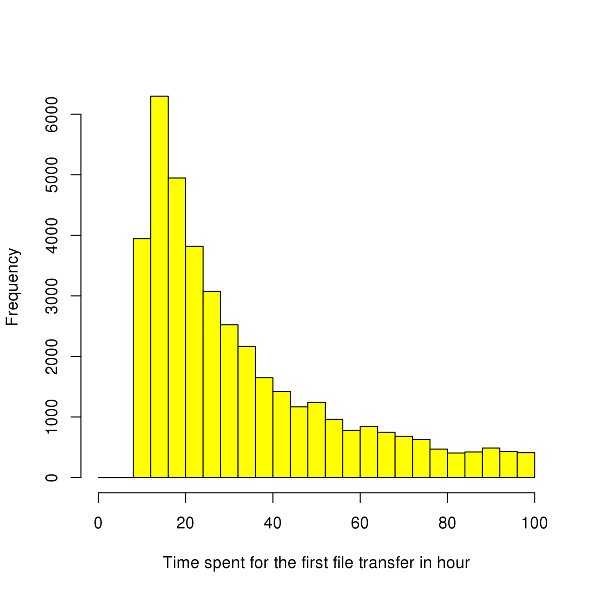
\includegraphics{Figures/figure-71.pdf}
\caption{Frequency histogram of the first file replica time (in hour)
  for the transfers tagged as being ``early-stuck'' according to
  eq.~\ref{eq:early-stuck}.}\label{fig:figure-7.1}
\end{figure}

These transfers are hence reported as stuck at 0\% completion for
hours as shown in fig.~\ref{fig:figure-7.1}, so it is far easier
to detect them with respect to any other latency type.

In addition, $SkewLast_{75}$ values (see eq.~\ref{eq:skewlast}) are
quite small while $Skew_{25}$ (see eq.~\ref{eq:skewlast}) have quite
large values in fig.~\ref{fig:figure-7.2} as expected.

\begin{figure}[htp]
\centering
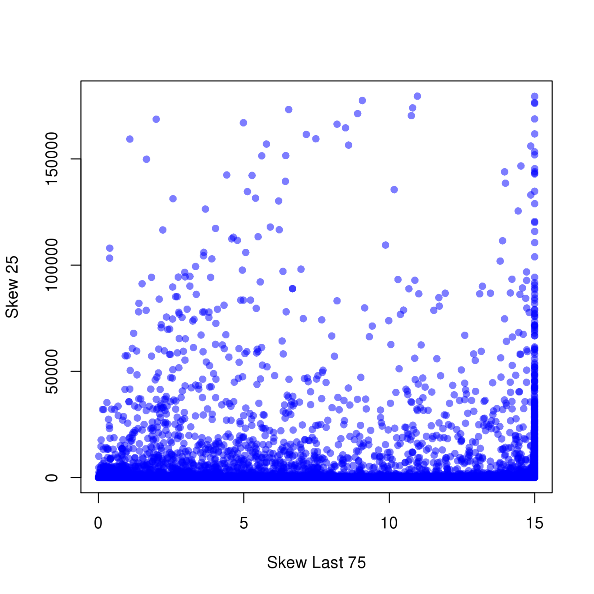
\includegraphics{Figures/figure-72.pdf}
\caption{$Skew_{25}$ versus $SkewLast_{75}$ as defined in
  eq.~\ref{eq:skew} and eq.~\ref{eq:skewlast}. For transfers tagged as
  being ``early-stuck'' according to
  eq.~\ref{eq:early-stuck}.}\label{fig:figure-7.2}
\end{figure}

The solution, however, is not straight-forward: it might require site
admin intervention at the source/destination site, or even central
operators/experts involvement. The price to pay if not promptly
identified is high: only a quick problem identification, attack and
fix can avoid to pile up delays and additional work load at a later
stage.
